\documentclass[12pt]{article}
\renewcommand{\thesection}{\Roman{section}} 
\renewcommand{\thesubsection}{\thesection.\Roman{subsection}}
\usepackage[tocindentauto]{tocstyle}
%\usetocstyle{KOMAlike} %the previous line resets it
\usepackage{natbib}
\usepackage{url}
\usepackage[utf8x]{inputenc}
\usepackage{amsmath}
\usepackage{graphicx}
\usepackage{verbatim}
\graphicspath{{images/}}
\usepackage{parskip}
\usepackage{fancyhdr}
\usepackage{vmargin}
\setmarginsrb{3 cm}{2.5 cm}{3 cm}{2.5 cm}{1 cm}{1.5 cm}{1 cm}{1.5 cm}
\usepackage{appendix}
\usepackage{listings} % For code importing
\usepackage{xcolor} % for setting colors
 %%%%%%%%%%%%%%%%%%%%%%%%%%%%%%%%%%%%%%%%%%%%%%%%%%%%%%%%%%%%%%%%%%%%%%%%%%%%%%%% 
%%% ~ Arduino Language - Arduino IDE Colors ~                                  %%%
%%%                                                                            %%%
%%% Kyle Rocha-Brownell | 10/2/2017 | No Licence                               %%%
%%% -------------------------------------------------------------------------- %%%
%%%                                                                            %%%
%%% Place this file in your working directory (next to the latex file you're   %%%
%%% working on).  To add it to your project, place:                            %%%
%%%     %%%%%%%%%%%%%%%%%%%%%%%%%%%%%%%%%%%%%%%%%%%%%%%%%%%%%%%%%%%%%%%%%%%%%%%%%%%%%%%% 
%%% ~ Arduino Language - Arduino IDE Colors ~                                  %%%
%%%                                                                            %%%
%%% Kyle Rocha-Brownell | 10/2/2017 | No Licence                               %%%
%%% -------------------------------------------------------------------------- %%%
%%%                                                                            %%%
%%% Place this file in your working directory (next to the latex file you're   %%%
%%% working on).  To add it to your project, place:                            %%%
%%%     %%%%%%%%%%%%%%%%%%%%%%%%%%%%%%%%%%%%%%%%%%%%%%%%%%%%%%%%%%%%%%%%%%%%%%%%%%%%%%%% 
%%% ~ Arduino Language - Arduino IDE Colors ~                                  %%%
%%%                                                                            %%%
%%% Kyle Rocha-Brownell | 10/2/2017 | No Licence                               %%%
%%% -------------------------------------------------------------------------- %%%
%%%                                                                            %%%
%%% Place this file in your working directory (next to the latex file you're   %%%
%%% working on).  To add it to your project, place:                            %%%
%%%    \input{arduinoLanguage.tex}                                             %%%
%%% somewhere before \begin{document} in your latex file.                      %%%
%%%                                                                            %%%
%%% In your document, place your arduino code between:                         %%%
%%%   \begin{lstlisting}[language=Arduino]                                     %%%
%%% and:                                                                       %%%
%%%   \end{lstlisting}                                                         %%%
%%%                                                                            %%%
%%% Or create your own style to add non-built-in functions and variables.      %%%
%%%                                                                            %%%
 %%%%%%%%%%%%%%%%%%%%%%%%%%%%%%%%%%%%%%%%%%%%%%%%%%%%%%%%%%%%%%%%%%%%%%%%%%%%%%%% 

\usepackage{color}
\usepackage{listings}    
\usepackage{courier}

%%% Define Custom IDE Colors %%%
\definecolor{arduinoGreen}    {rgb} {0.17, 0.43, 0.01}
\definecolor{arduinoGrey}     {rgb} {0.47, 0.47, 0.33}
\definecolor{arduinoOrange}   {rgb} {0.8 , 0.4 , 0   }
\definecolor{arduinoBlue}     {rgb} {0.01, 0.61, 0.98}
\definecolor{arduinoDarkBlue} {rgb} {0.0 , 0.2 , 0.5 }

%%% Define Arduino Language %%%
\lstdefinelanguage{Arduino}{
  language=C++, % begin with default C++ settings 
%
%
  %%% Keyword Color Group 1 %%%  (called KEYWORD3 by arduino)
  keywordstyle=\color{arduinoGreen},   
  deletekeywords={  % remove all arduino keywords that might be in c++
                break, case, override, final, continue, default, do, else, for, 
                if, return, goto, switch, throw, try, while, setup, loop, export, 
                not, or, and, xor, include, define, elif, else, error, if, ifdef, 
                ifndef, pragma, warning,
                HIGH, LOW, INPUT, INPUT_PULLUP, OUTPUT, DEC, BIN, HEX, OCT, PI, 
                HALF_PI, TWO_PI, LSBFIRST, MSBFIRST, CHANGE, FALLING, RISING, 
                DEFAULT, EXTERNAL, INTERNAL, INTERNAL1V1, INTERNAL2V56, LED_BUILTIN, 
                LED_BUILTIN_RX, LED_BUILTIN_TX, DIGITAL_MESSAGE, FIRMATA_STRING, 
                ANALOG_MESSAGE, REPORT_DIGITAL, REPORT_ANALOG, SET_PIN_MODE, 
                SYSTEM_RESET, SYSEX_START, auto, int8_t, int16_t, int32_t, int64_t, 
                uint8_t, uint16_t, uint32_t, uint64_t, char16_t, char32_t, operator, 
                enum, delete, bool, boolean, byte, char, const, false, float, double, 
                null, NULL, int, long, new, private, protected, public, short, 
                signed, static, volatile, String, void, true, unsigned, word, array, 
                sizeof, dynamic_cast, typedef, const_cast, struct, static_cast, union, 
                friend, extern, class, reinterpret_cast, register, explicit, inline, 
                _Bool, complex, _Complex, _Imaginary, atomic_bool, atomic_char, 
                atomic_schar, atomic_uchar, atomic_short, atomic_ushort, atomic_int, 
                atomic_uint, atomic_long, atomic_ulong, atomic_llong, atomic_ullong, 
                virtual, PROGMEM,
                Serial, Serial1, Serial2, Serial3, SerialUSB, Keyboard, Mouse,
                abs, acos, asin, atan, atan2, ceil, constrain, cos, degrees, exp, 
                floor, log, map, max, min, radians, random, randomSeed, round, sin, 
                sq, sqrt, tan, pow, bitRead, bitWrite, bitSet, bitClear, bit, 
                highByte, lowByte, analogReference, analogRead, 
                analogReadResolution, analogWrite, analogWriteResolution, 
                attachInterrupt, detachInterrupt, digitalPinToInterrupt, delay, 
                delayMicroseconds, digitalWrite, digitalRead, interrupts, millis, 
                micros, noInterrupts, noTone, pinMode, pulseIn, pulseInLong, shiftIn, 
                shiftOut, tone, yield, Stream, begin, end, peek, read, print, 
                println, available, availableForWrite, flush, setTimeout, find, 
                findUntil, parseInt, parseFloat, readBytes, readBytesUntil, readString, 
                readStringUntil, trim, toUpperCase, toLowerCase, charAt, compareTo, 
                concat, endsWith, startsWith, equals, equalsIgnoreCase, getBytes, 
                indexOf, lastIndexOf, length, replace, setCharAt, substring, 
                toCharArray, toInt, press, release, releaseAll, accept, click, move, 
                isPressed, isAlphaNumeric, isAlpha, isAscii, isWhitespace, isControl, 
                isDigit, isGraph, isLowerCase, isPrintable, isPunct, isSpace, 
                isUpperCase, isHexadecimalDigit, 
                }, 
  morekeywords={   % add arduino structures to group 1
                break, case, override, final, continue, default, do, else, for, 
                if, return, goto, switch, throw, try, while, setup, loop, export, 
                not, or, and, xor, include, define, elif, else, error, if, ifdef, 
                ifndef, pragma, warning,
                }, 
% 
%
  %%% Keyword Color Group 2 %%%  (called LITERAL1 by arduino)
  keywordstyle=[2]\color{arduinoBlue},   
  keywords=[2]{   % add variables and dataTypes as 2nd group  
                HIGH, LOW, INPUT, INPUT_PULLUP, OUTPUT, DEC, BIN, HEX, OCT, PI, 
                HALF_PI, TWO_PI, LSBFIRST, MSBFIRST, CHANGE, FALLING, RISING, 
                DEFAULT, EXTERNAL, INTERNAL, INTERNAL1V1, INTERNAL2V56, LED_BUILTIN, 
                LED_BUILTIN_RX, LED_BUILTIN_TX, DIGITAL_MESSAGE, FIRMATA_STRING, 
                ANALOG_MESSAGE, REPORT_DIGITAL, REPORT_ANALOG, SET_PIN_MODE, 
                SYSTEM_RESET, SYSEX_START, auto, int8_t, int16_t, int32_t, int64_t, 
                uint8_t, uint16_t, uint32_t, uint64_t, char16_t, char32_t, operator, 
                enum, delete, bool, boolean, byte, char, const, false, float, double, 
                null, NULL, int, long, new, private, protected, public, short, 
                signed, static, volatile, String, void, true, unsigned, word, array, 
                sizeof, dynamic_cast, typedef, const_cast, struct, static_cast, union, 
                friend, extern, class, reinterpret_cast, register, explicit, inline, 
                _Bool, complex, _Complex, _Imaginary, atomic_bool, atomic_char, 
                atomic_schar, atomic_uchar, atomic_short, atomic_ushort, atomic_int, 
                atomic_uint, atomic_long, atomic_ulong, atomic_llong, atomic_ullong, 
                virtual, PROGMEM,
                },  
% 
%
  %%% Keyword Color Group 3 %%%  (called KEYWORD1 by arduino)
  keywordstyle=[3]\bfseries\color{arduinoOrange},
  keywords=[3]{  % add built-in functions as a 3rd group
                Serial, Serial1, Serial2, Serial3, SerialUSB, Keyboard, Mouse,
                },      
%
%
  %%% Keyword Color Group 4 %%%  (called KEYWORD2 by arduino)
  keywordstyle=[4]\color{arduinoOrange},
  keywords=[4]{  % add more built-in functions as a 4th group
                abs, acos, asin, atan, atan2, ceil, constrain, cos, degrees, exp, 
                floor, log, map, max, min, radians, random, randomSeed, round, sin, 
                sq, sqrt, tan, pow, bitRead, bitWrite, bitSet, bitClear, bit, 
                highByte, lowByte, analogReference, analogRead, 
                analogReadResolution, analogWrite, analogWriteResolution, 
                attachInterrupt, detachInterrupt, digitalPinToInterrupt, delay, 
                delayMicroseconds, digitalWrite, digitalRead, interrupts, millis, 
                micros, noInterrupts, noTone, pinMode, pulseIn, pulseInLong, shiftIn, 
                shiftOut, tone, yield, Stream, begin, end, peek, read, print, 
                println, available, availableForWrite, flush, setTimeout, find, 
                findUntil, parseInt, parseFloat, readBytes, readBytesUntil, readString, 
                readStringUntil, trim, toUpperCase, toLowerCase, charAt, compareTo, 
                concat, endsWith, startsWith, equals, equalsIgnoreCase, getBytes, 
                indexOf, lastIndexOf, length, replace, setCharAt, substring, 
                toCharArray, toInt, press, release, releaseAll, accept, click, move, 
                isPressed, isAlphaNumeric, isAlpha, isAscii, isWhitespace, isControl, 
                isDigit, isGraph, isLowerCase, isPrintable, isPunct, isSpace, 
                isUpperCase, isHexadecimalDigit, 
                },      
%
%
  %%% Set Other Colors %%%
  stringstyle=\color{arduinoDarkBlue},    
  commentstyle=\color{arduinoGrey},    
%          
%   
  %%%% Line Numbering %%%%
   numbers=left,                    
  numbersep=5pt,                   
  numberstyle=\color{arduinoGrey},    
  %stepnumber=2,                      % show every 2 line numbers
%
%
  %%%% Code Box Style %%%%
  breaklines=true,                    % wordwrapping
  tabsize=2,         
  basicstyle=\ttfamily  
}                                             %%%
%%% somewhere before \begin{document} in your latex file.                      %%%
%%%                                                                            %%%
%%% In your document, place your arduino code between:                         %%%
%%%   \begin{lstlisting}[language=Arduino]                                     %%%
%%% and:                                                                       %%%
%%%   \end{lstlisting}                                                         %%%
%%%                                                                            %%%
%%% Or create your own style to add non-built-in functions and variables.      %%%
%%%                                                                            %%%
 %%%%%%%%%%%%%%%%%%%%%%%%%%%%%%%%%%%%%%%%%%%%%%%%%%%%%%%%%%%%%%%%%%%%%%%%%%%%%%%% 

\usepackage{color}
\usepackage{listings}    
\usepackage{courier}

%%% Define Custom IDE Colors %%%
\definecolor{arduinoGreen}    {rgb} {0.17, 0.43, 0.01}
\definecolor{arduinoGrey}     {rgb} {0.47, 0.47, 0.33}
\definecolor{arduinoOrange}   {rgb} {0.8 , 0.4 , 0   }
\definecolor{arduinoBlue}     {rgb} {0.01, 0.61, 0.98}
\definecolor{arduinoDarkBlue} {rgb} {0.0 , 0.2 , 0.5 }

%%% Define Arduino Language %%%
\lstdefinelanguage{Arduino}{
  language=C++, % begin with default C++ settings 
%
%
  %%% Keyword Color Group 1 %%%  (called KEYWORD3 by arduino)
  keywordstyle=\color{arduinoGreen},   
  deletekeywords={  % remove all arduino keywords that might be in c++
                break, case, override, final, continue, default, do, else, for, 
                if, return, goto, switch, throw, try, while, setup, loop, export, 
                not, or, and, xor, include, define, elif, else, error, if, ifdef, 
                ifndef, pragma, warning,
                HIGH, LOW, INPUT, INPUT_PULLUP, OUTPUT, DEC, BIN, HEX, OCT, PI, 
                HALF_PI, TWO_PI, LSBFIRST, MSBFIRST, CHANGE, FALLING, RISING, 
                DEFAULT, EXTERNAL, INTERNAL, INTERNAL1V1, INTERNAL2V56, LED_BUILTIN, 
                LED_BUILTIN_RX, LED_BUILTIN_TX, DIGITAL_MESSAGE, FIRMATA_STRING, 
                ANALOG_MESSAGE, REPORT_DIGITAL, REPORT_ANALOG, SET_PIN_MODE, 
                SYSTEM_RESET, SYSEX_START, auto, int8_t, int16_t, int32_t, int64_t, 
                uint8_t, uint16_t, uint32_t, uint64_t, char16_t, char32_t, operator, 
                enum, delete, bool, boolean, byte, char, const, false, float, double, 
                null, NULL, int, long, new, private, protected, public, short, 
                signed, static, volatile, String, void, true, unsigned, word, array, 
                sizeof, dynamic_cast, typedef, const_cast, struct, static_cast, union, 
                friend, extern, class, reinterpret_cast, register, explicit, inline, 
                _Bool, complex, _Complex, _Imaginary, atomic_bool, atomic_char, 
                atomic_schar, atomic_uchar, atomic_short, atomic_ushort, atomic_int, 
                atomic_uint, atomic_long, atomic_ulong, atomic_llong, atomic_ullong, 
                virtual, PROGMEM,
                Serial, Serial1, Serial2, Serial3, SerialUSB, Keyboard, Mouse,
                abs, acos, asin, atan, atan2, ceil, constrain, cos, degrees, exp, 
                floor, log, map, max, min, radians, random, randomSeed, round, sin, 
                sq, sqrt, tan, pow, bitRead, bitWrite, bitSet, bitClear, bit, 
                highByte, lowByte, analogReference, analogRead, 
                analogReadResolution, analogWrite, analogWriteResolution, 
                attachInterrupt, detachInterrupt, digitalPinToInterrupt, delay, 
                delayMicroseconds, digitalWrite, digitalRead, interrupts, millis, 
                micros, noInterrupts, noTone, pinMode, pulseIn, pulseInLong, shiftIn, 
                shiftOut, tone, yield, Stream, begin, end, peek, read, print, 
                println, available, availableForWrite, flush, setTimeout, find, 
                findUntil, parseInt, parseFloat, readBytes, readBytesUntil, readString, 
                readStringUntil, trim, toUpperCase, toLowerCase, charAt, compareTo, 
                concat, endsWith, startsWith, equals, equalsIgnoreCase, getBytes, 
                indexOf, lastIndexOf, length, replace, setCharAt, substring, 
                toCharArray, toInt, press, release, releaseAll, accept, click, move, 
                isPressed, isAlphaNumeric, isAlpha, isAscii, isWhitespace, isControl, 
                isDigit, isGraph, isLowerCase, isPrintable, isPunct, isSpace, 
                isUpperCase, isHexadecimalDigit, 
                }, 
  morekeywords={   % add arduino structures to group 1
                break, case, override, final, continue, default, do, else, for, 
                if, return, goto, switch, throw, try, while, setup, loop, export, 
                not, or, and, xor, include, define, elif, else, error, if, ifdef, 
                ifndef, pragma, warning,
                }, 
% 
%
  %%% Keyword Color Group 2 %%%  (called LITERAL1 by arduino)
  keywordstyle=[2]\color{arduinoBlue},   
  keywords=[2]{   % add variables and dataTypes as 2nd group  
                HIGH, LOW, INPUT, INPUT_PULLUP, OUTPUT, DEC, BIN, HEX, OCT, PI, 
                HALF_PI, TWO_PI, LSBFIRST, MSBFIRST, CHANGE, FALLING, RISING, 
                DEFAULT, EXTERNAL, INTERNAL, INTERNAL1V1, INTERNAL2V56, LED_BUILTIN, 
                LED_BUILTIN_RX, LED_BUILTIN_TX, DIGITAL_MESSAGE, FIRMATA_STRING, 
                ANALOG_MESSAGE, REPORT_DIGITAL, REPORT_ANALOG, SET_PIN_MODE, 
                SYSTEM_RESET, SYSEX_START, auto, int8_t, int16_t, int32_t, int64_t, 
                uint8_t, uint16_t, uint32_t, uint64_t, char16_t, char32_t, operator, 
                enum, delete, bool, boolean, byte, char, const, false, float, double, 
                null, NULL, int, long, new, private, protected, public, short, 
                signed, static, volatile, String, void, true, unsigned, word, array, 
                sizeof, dynamic_cast, typedef, const_cast, struct, static_cast, union, 
                friend, extern, class, reinterpret_cast, register, explicit, inline, 
                _Bool, complex, _Complex, _Imaginary, atomic_bool, atomic_char, 
                atomic_schar, atomic_uchar, atomic_short, atomic_ushort, atomic_int, 
                atomic_uint, atomic_long, atomic_ulong, atomic_llong, atomic_ullong, 
                virtual, PROGMEM,
                },  
% 
%
  %%% Keyword Color Group 3 %%%  (called KEYWORD1 by arduino)
  keywordstyle=[3]\bfseries\color{arduinoOrange},
  keywords=[3]{  % add built-in functions as a 3rd group
                Serial, Serial1, Serial2, Serial3, SerialUSB, Keyboard, Mouse,
                },      
%
%
  %%% Keyword Color Group 4 %%%  (called KEYWORD2 by arduino)
  keywordstyle=[4]\color{arduinoOrange},
  keywords=[4]{  % add more built-in functions as a 4th group
                abs, acos, asin, atan, atan2, ceil, constrain, cos, degrees, exp, 
                floor, log, map, max, min, radians, random, randomSeed, round, sin, 
                sq, sqrt, tan, pow, bitRead, bitWrite, bitSet, bitClear, bit, 
                highByte, lowByte, analogReference, analogRead, 
                analogReadResolution, analogWrite, analogWriteResolution, 
                attachInterrupt, detachInterrupt, digitalPinToInterrupt, delay, 
                delayMicroseconds, digitalWrite, digitalRead, interrupts, millis, 
                micros, noInterrupts, noTone, pinMode, pulseIn, pulseInLong, shiftIn, 
                shiftOut, tone, yield, Stream, begin, end, peek, read, print, 
                println, available, availableForWrite, flush, setTimeout, find, 
                findUntil, parseInt, parseFloat, readBytes, readBytesUntil, readString, 
                readStringUntil, trim, toUpperCase, toLowerCase, charAt, compareTo, 
                concat, endsWith, startsWith, equals, equalsIgnoreCase, getBytes, 
                indexOf, lastIndexOf, length, replace, setCharAt, substring, 
                toCharArray, toInt, press, release, releaseAll, accept, click, move, 
                isPressed, isAlphaNumeric, isAlpha, isAscii, isWhitespace, isControl, 
                isDigit, isGraph, isLowerCase, isPrintable, isPunct, isSpace, 
                isUpperCase, isHexadecimalDigit, 
                },      
%
%
  %%% Set Other Colors %%%
  stringstyle=\color{arduinoDarkBlue},    
  commentstyle=\color{arduinoGrey},    
%          
%   
  %%%% Line Numbering %%%%
   numbers=left,                    
  numbersep=5pt,                   
  numberstyle=\color{arduinoGrey},    
  %stepnumber=2,                      % show every 2 line numbers
%
%
  %%%% Code Box Style %%%%
  breaklines=true,                    % wordwrapping
  tabsize=2,         
  basicstyle=\ttfamily  
}                                             %%%
%%% somewhere before \begin{document} in your latex file.                      %%%
%%%                                                                            %%%
%%% In your document, place your arduino code between:                         %%%
%%%   \begin{lstlisting}[language=Arduino]                                     %%%
%%% and:                                                                       %%%
%%%   \end{lstlisting}                                                         %%%
%%%                                                                            %%%
%%% Or create your own style to add non-built-in functions and variables.      %%%
%%%                                                                            %%%
 %%%%%%%%%%%%%%%%%%%%%%%%%%%%%%%%%%%%%%%%%%%%%%%%%%%%%%%%%%%%%%%%%%%%%%%%%%%%%%%% 

\usepackage{color}
\usepackage{listings}    
\usepackage{courier}

%%% Define Custom IDE Colors %%%
\definecolor{arduinoGreen}    {rgb} {0.17, 0.43, 0.01}
\definecolor{arduinoGrey}     {rgb} {0.47, 0.47, 0.33}
\definecolor{arduinoOrange}   {rgb} {0.8 , 0.4 , 0   }
\definecolor{arduinoBlue}     {rgb} {0.01, 0.61, 0.98}
\definecolor{arduinoDarkBlue} {rgb} {0.0 , 0.2 , 0.5 }

%%% Define Arduino Language %%%
\lstdefinelanguage{Arduino}{
  language=C++, % begin with default C++ settings 
%
%
  %%% Keyword Color Group 1 %%%  (called KEYWORD3 by arduino)
  keywordstyle=\color{arduinoGreen},   
  deletekeywords={  % remove all arduino keywords that might be in c++
                break, case, override, final, continue, default, do, else, for, 
                if, return, goto, switch, throw, try, while, setup, loop, export, 
                not, or, and, xor, include, define, elif, else, error, if, ifdef, 
                ifndef, pragma, warning,
                HIGH, LOW, INPUT, INPUT_PULLUP, OUTPUT, DEC, BIN, HEX, OCT, PI, 
                HALF_PI, TWO_PI, LSBFIRST, MSBFIRST, CHANGE, FALLING, RISING, 
                DEFAULT, EXTERNAL, INTERNAL, INTERNAL1V1, INTERNAL2V56, LED_BUILTIN, 
                LED_BUILTIN_RX, LED_BUILTIN_TX, DIGITAL_MESSAGE, FIRMATA_STRING, 
                ANALOG_MESSAGE, REPORT_DIGITAL, REPORT_ANALOG, SET_PIN_MODE, 
                SYSTEM_RESET, SYSEX_START, auto, int8_t, int16_t, int32_t, int64_t, 
                uint8_t, uint16_t, uint32_t, uint64_t, char16_t, char32_t, operator, 
                enum, delete, bool, boolean, byte, char, const, false, float, double, 
                null, NULL, int, long, new, private, protected, public, short, 
                signed, static, volatile, String, void, true, unsigned, word, array, 
                sizeof, dynamic_cast, typedef, const_cast, struct, static_cast, union, 
                friend, extern, class, reinterpret_cast, register, explicit, inline, 
                _Bool, complex, _Complex, _Imaginary, atomic_bool, atomic_char, 
                atomic_schar, atomic_uchar, atomic_short, atomic_ushort, atomic_int, 
                atomic_uint, atomic_long, atomic_ulong, atomic_llong, atomic_ullong, 
                virtual, PROGMEM,
                Serial, Serial1, Serial2, Serial3, SerialUSB, Keyboard, Mouse,
                abs, acos, asin, atan, atan2, ceil, constrain, cos, degrees, exp, 
                floor, log, map, max, min, radians, random, randomSeed, round, sin, 
                sq, sqrt, tan, pow, bitRead, bitWrite, bitSet, bitClear, bit, 
                highByte, lowByte, analogReference, analogRead, 
                analogReadResolution, analogWrite, analogWriteResolution, 
                attachInterrupt, detachInterrupt, digitalPinToInterrupt, delay, 
                delayMicroseconds, digitalWrite, digitalRead, interrupts, millis, 
                micros, noInterrupts, noTone, pinMode, pulseIn, pulseInLong, shiftIn, 
                shiftOut, tone, yield, Stream, begin, end, peek, read, print, 
                println, available, availableForWrite, flush, setTimeout, find, 
                findUntil, parseInt, parseFloat, readBytes, readBytesUntil, readString, 
                readStringUntil, trim, toUpperCase, toLowerCase, charAt, compareTo, 
                concat, endsWith, startsWith, equals, equalsIgnoreCase, getBytes, 
                indexOf, lastIndexOf, length, replace, setCharAt, substring, 
                toCharArray, toInt, press, release, releaseAll, accept, click, move, 
                isPressed, isAlphaNumeric, isAlpha, isAscii, isWhitespace, isControl, 
                isDigit, isGraph, isLowerCase, isPrintable, isPunct, isSpace, 
                isUpperCase, isHexadecimalDigit, 
                }, 
  morekeywords={   % add arduino structures to group 1
                break, case, override, final, continue, default, do, else, for, 
                if, return, goto, switch, throw, try, while, setup, loop, export, 
                not, or, and, xor, include, define, elif, else, error, if, ifdef, 
                ifndef, pragma, warning,
                }, 
% 
%
  %%% Keyword Color Group 2 %%%  (called LITERAL1 by arduino)
  keywordstyle=[2]\color{arduinoBlue},   
  keywords=[2]{   % add variables and dataTypes as 2nd group  
                HIGH, LOW, INPUT, INPUT_PULLUP, OUTPUT, DEC, BIN, HEX, OCT, PI, 
                HALF_PI, TWO_PI, LSBFIRST, MSBFIRST, CHANGE, FALLING, RISING, 
                DEFAULT, EXTERNAL, INTERNAL, INTERNAL1V1, INTERNAL2V56, LED_BUILTIN, 
                LED_BUILTIN_RX, LED_BUILTIN_TX, DIGITAL_MESSAGE, FIRMATA_STRING, 
                ANALOG_MESSAGE, REPORT_DIGITAL, REPORT_ANALOG, SET_PIN_MODE, 
                SYSTEM_RESET, SYSEX_START, auto, int8_t, int16_t, int32_t, int64_t, 
                uint8_t, uint16_t, uint32_t, uint64_t, char16_t, char32_t, operator, 
                enum, delete, bool, boolean, byte, char, const, false, float, double, 
                null, NULL, int, long, new, private, protected, public, short, 
                signed, static, volatile, String, void, true, unsigned, word, array, 
                sizeof, dynamic_cast, typedef, const_cast, struct, static_cast, union, 
                friend, extern, class, reinterpret_cast, register, explicit, inline, 
                _Bool, complex, _Complex, _Imaginary, atomic_bool, atomic_char, 
                atomic_schar, atomic_uchar, atomic_short, atomic_ushort, atomic_int, 
                atomic_uint, atomic_long, atomic_ulong, atomic_llong, atomic_ullong, 
                virtual, PROGMEM,
                },  
% 
%
  %%% Keyword Color Group 3 %%%  (called KEYWORD1 by arduino)
  keywordstyle=[3]\bfseries\color{arduinoOrange},
  keywords=[3]{  % add built-in functions as a 3rd group
                Serial, Serial1, Serial2, Serial3, SerialUSB, Keyboard, Mouse,
                },      
%
%
  %%% Keyword Color Group 4 %%%  (called KEYWORD2 by arduino)
  keywordstyle=[4]\color{arduinoOrange},
  keywords=[4]{  % add more built-in functions as a 4th group
                abs, acos, asin, atan, atan2, ceil, constrain, cos, degrees, exp, 
                floor, log, map, max, min, radians, random, randomSeed, round, sin, 
                sq, sqrt, tan, pow, bitRead, bitWrite, bitSet, bitClear, bit, 
                highByte, lowByte, analogReference, analogRead, 
                analogReadResolution, analogWrite, analogWriteResolution, 
                attachInterrupt, detachInterrupt, digitalPinToInterrupt, delay, 
                delayMicroseconds, digitalWrite, digitalRead, interrupts, millis, 
                micros, noInterrupts, noTone, pinMode, pulseIn, pulseInLong, shiftIn, 
                shiftOut, tone, yield, Stream, begin, end, peek, read, print, 
                println, available, availableForWrite, flush, setTimeout, find, 
                findUntil, parseInt, parseFloat, readBytes, readBytesUntil, readString, 
                readStringUntil, trim, toUpperCase, toLowerCase, charAt, compareTo, 
                concat, endsWith, startsWith, equals, equalsIgnoreCase, getBytes, 
                indexOf, lastIndexOf, length, replace, setCharAt, substring, 
                toCharArray, toInt, press, release, releaseAll, accept, click, move, 
                isPressed, isAlphaNumeric, isAlpha, isAscii, isWhitespace, isControl, 
                isDigit, isGraph, isLowerCase, isPrintable, isPunct, isSpace, 
                isUpperCase, isHexadecimalDigit, 
                },      
%
%
  %%% Set Other Colors %%%
  stringstyle=\color{arduinoDarkBlue},    
  commentstyle=\color{arduinoGrey},    
%          
%   
  %%%% Line Numbering %%%%
   numbers=left,                    
  numbersep=5pt,                   
  numberstyle=\color{arduinoGrey},    
  %stepnumber=2,                      % show every 2 line numbers
%
%
  %%%% Code Box Style %%%%
  breaklines=true,                    % wordwrapping
  tabsize=2,         
  basicstyle=\ttfamily  
}  

%\makeatletter
%\let\thetitle\@title

%\let\thedate\@date
%\makeatother

%\pagestyle{fancy}
%\fancyhf{}
%\rhead{\theauthor}
%\lhead{\thetitle}
%\cfoot{\thepage}

\begin{document}
\title{Project Report}
%%%%%%%%%%%%%%%%%%%%%%%%%%%%%%%%%%%%%%%%%%%%%%%%%%%%%%%%%%%%%%%%%%%%%%%%%%%%%%%%%%%%%%%%%

\begin{titlepage}
	\centering
    \vspace*{0.5 cm}
    
\includegraphics[scale = 0.11]{isu_seal.png}\\[1.0 cm]	% University Logo
    \textsc{\LARGE IOWA STATE UNIVERSITY}\\[2.0 cm]
    \textsc{\large AEROSPACE ENGINEERING DEPARTMENT}\\[0.2 cm]
    \textsc{\large Computational Techniques for Aerospace Design}\\[0.2 cm]
	\textsc{\Large AERE 361}\\[0.5 cm]				% Course Code
	\textsc{\Large Project Report}\\[0.2 cm]
	\textsc{\Large \#include <EpicTeamName.h>}\\[0.2 cm]
	\rule{\linewidth}{0.2 mm} \\[0.4 cm]
	%{ \huge \bfseries \thetitle}\\
	
	\begin{minipage}{0.8\textwidth}
		
			\begin{flushleft} 
			\emph{Team Member Names :} \\
			Gill, Jarod\linebreak
			Hingst, Charles\linebreak
			Poppinga, Ashley\linebreak
			Swayne, Logan\linebreak
			
		\end{flushleft}
	\end{minipage}\\[2 cm]
	
	\vfill 
6

	
\end{titlepage}

%%%%%%%%%%%%%%%%%%%%%%%%%%%%%%%%%%%%%%%%%%%%%%%%%%%%%%%%%%%%%%%%%%%%%%%%%%%%%%%%%%%%%%%%%
%\maketitle
\tableofcontents
\pagebreak
%%%%%%%%%%%%%%%%%%%%%%%%%%%%%%%%%%%%%%%%%%%%%%%%%%%%%%%%%%%%%%%%%%%%%%%%%%%%%%%%%%%%%%%%%

\section{ABSTRACT} % JAROD WRITE LAST!!!
% This is your abstract.  It is a short summary of what your report will cover.  You should keep your abstract to 250 words or less.  Use this to ``hook in'' your reader.
Are you struggling with boredom in isolation during the COVID-19 pandemic? Need something more interactive and challenging rather than just pure entertainment? Well, our team has developed a solution inspired from a classic memory game that provides short, fun games and utilizes a different interface: the Circuit Playground Express. This report will cover the various features implemented in our design, and how they the solve the problem. It will also include how we reached our final design solution, a game-play walk through, and the current status of our project. The report will conclude with some final remarks from our team, and afterwords the source code for our project.

\section{INTRODUCTION} % JAROD
% Introduce your project.  Brief summary of what it does and why you are doing this.  Should be 1-2 paragraphs.  This can be similar to what you have in your proposal, but if anything changed while working on the project, then make sure it is also reflected here.

In 1978, a simple interactive memory game called "Simon" was released  \cite{Edwards}, and it would become "a pivotal part of the 1980s electronic-toy craze" \cite{Townshend}. For our final project, we designed and developed an adaptation of the Simon device utilizing a Circuit Playground Express. This game provides a randomized sequence of inputs, introducing them one by one, in a designated order. The player will then repeat the growing sequence repeatedly until the victory condition is met, which will be a set sequence length determined by the player's difficulty level selection. 

\section{FEATURES} % ASHLEY
%%% List here all the features that your device has.  As mentioned in the writeup, you should have at least 3 major features.  Again, if any of  your features changed from your project proposal, then make sure it is updated here.  List all of the features that you actually implemented first.  You can cover features you did not implement in your lessons learned section.

The three major features of the Simon device are its LED display, sound indication, and difficulty selection. These features were mentioned in the initial project proposal, but were developed to be more complex than originally intended. The LED lights and sounds were intended to signal collection of user input and a win/lose condition. We extended this capability to operate upon startup as well as to indicate the desired color sequence. Since the submission of the project proposal, a difficulty feature was also added to allow the user to speed up and lengthen the sequence of the game. Each of these features were tweaked in the final stages of development to make the game more user-friendly.

\section{PROBLEM STATEMENT} % ASHLEY
%Here you will go into more detail on what problem you solved or addressed with your project.  You should discuss what the problem is and briefly introduce how you plan to solve it. Also, don't forget you should be referencing at least 1 sources.\cite{einstein}. You of course can cite additional sources as well.\citep{dirac}

The COVID-19 pandemic has forced many into isolation with little to do. A study featured in the European Journal of Psychotraumatology concluded that boredom during the pandemic has contributed to the development of conditions such as depression, anxiety, and stress in respondents \cite{Chao}. This study also found that these conditions caused participants to question the meaning of life \cite{Chao}. There is a demonstrated need for a device that allows those in isolation to stay mentally engaged and entertained during this pandemic.

\section{PROBLEM SOLUTION}
%Here, you go into detail what your solution to the problem is.  I expect that this will have several subsections and you should breakout each area.  You should include any graphics as relevant as well and reference them like Figure \ref{fig:cpx}.
%\begin{figure}[!t]
%\centering
%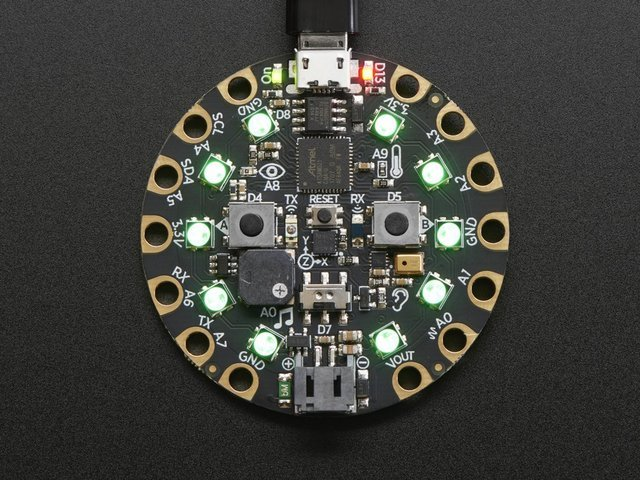
\includegraphics[width=4.5in]{cpx01.jpg}
%\caption{This is the circuit playground express}
%\label{fig:cpx}
%\end{figure}
%Again, cite any sources that you have.  If you took snippets of code or found a paper that discusses on how to do something, then you need to cite it.  For this final project report, I am expecting at least 3 sources cited.  One will probably be what you had in your problem statement from your proposal.  

The Simon device starts by first having the user select a level of difficulty for the game.  When the Slideswitch is in the left position, the user is able to choose a level of difficulty (1 Easiest - 10 Hardest) by pushing the right or left buttons.  To select a harder difficulty the user presses the right button (+1 difficulty) and to select an easier difficulty the user presses the left button (-1 difficulty).  Once satisfied with their selection, the user must slide the Slideswitch to the right position to be able to initiate the start of the game.

(Note: The default difficulty setting is 1 [Easiest].  If the user starts the game without setting the difficulty, the game will be in it's easiest mode.)

To start the game, the user must simultaneously press the left and right buttons.  This will take the device into the game loop where the it will display a pattern via the LEDs and the user must then touch the correct sections of the device in the same displayed order.  Each round, the device will display the last rounds pattern plus an additional section to be added to the pattern.  The user will be expected to input the entire pattern plus the additional displayed section added to the pattern.  To indicate the device has received an input from the user, it will light up in the touched section and play the section tone.  The time the patterns and new sections are displayed by the device will decrease with each round.\\

If the user makes an error and touches a section inconsistent with the pattern, the game will immediately end in Defeat.  The device will flash three times in the correct pattern section, play the defeat audio, and reset.  If the user is able to complete all of the patterns in the correct order for each round (based on the level of difficulty) the game will end in Victory and display a multitude of colors via the LEDs while music plays via the audio. The flow chart for this gameplay can be seen in Figure 1.

\begin{figure}[]
    \centering
    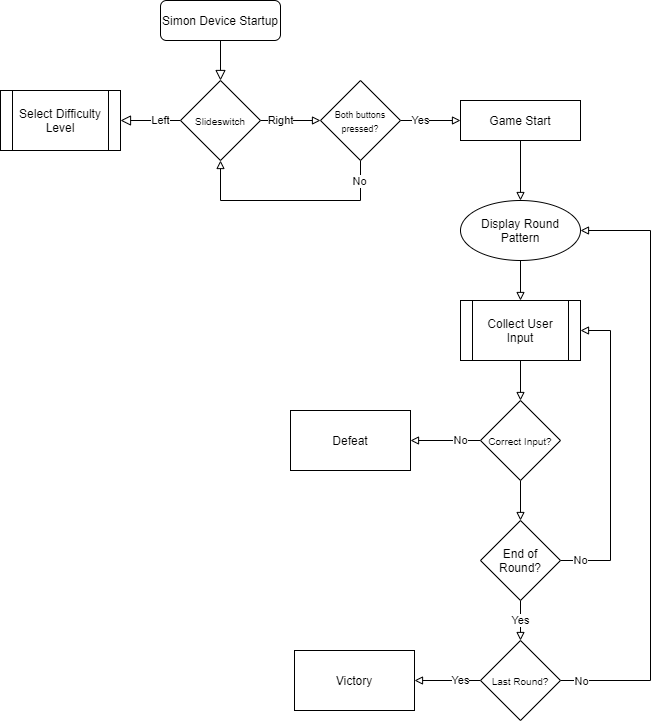
\includegraphics[width = 0.8\textwidth]{AERE_361_Project_Gameplay.png}
    \caption{Gameplay Diagram}
    \label{fig:gameplay}
\end{figure}

\subsection{Code Development} % LOGAN
%Pre-planning
Prior to development, it was important to understand the desired flow of the game. How does a game start? How is the pattern displayed to the user? How does the user match the pattern? What happens if the user enters an incorrect pattern? Does the game display anything special if the user wins? All of these questions and many more were asked, and from it, a clear vision of the game was developed.
\vspace*{0.5cm}
\\
%General Workflow of Code Development
Once the vision of the game was clear, each feature was broken down into its own smaller building blocks. This allowed for intermediate testing as each feature was added. The process of coding a feature, adding it to the main game script, and testing was repeated until all features were implemented and operating properly.
\subsubsection{Development of Basic Features}
%Starting the Game
The first feature that was developed was the start game condition. Once the circuit playground express was given power, it enters a while 1 == 1 loop that continuously checks if both buttons are pressed. If they are, then the game illuminates all ten LEDs green for one second then enters the game execution loop. This was the first building block.
\vspace*{0.5cm}
\\
%Displaying the Pattern
Next, code was needed to create a random pattern and display the pattern. To do this, the random function was used in a for loop to assign random numbers ranging from 1 to 4 to a vector that contained the pattern. In total, the pattern is equal to the maximum number of rounds in the game. It was found that the random function needed to first be seeded; otherwise, the random function would produce the same sequence of "random" numbers each time. The randomSeed function was used in conjunction with noise provided by one of the capacitive touch sensors to generate truly random numbers. Now that the pattern was defined, it needed to be displayed to the user. To do this, a for loop was created to iterate through the pattern vector, starting at pattern one and going until the number of patterns displayed matches the round number. Within each iteration, there are four if/else if statements that illuminate the LEDs (with the correct color within the setPixelColor function and sound within the playTone function) in the quadrant designated by the pattern vector. Refer to Figure \ref{fig:LED_Quadrants} for further information on the four quadrants. 
\begin{figure}[]
    \centering
    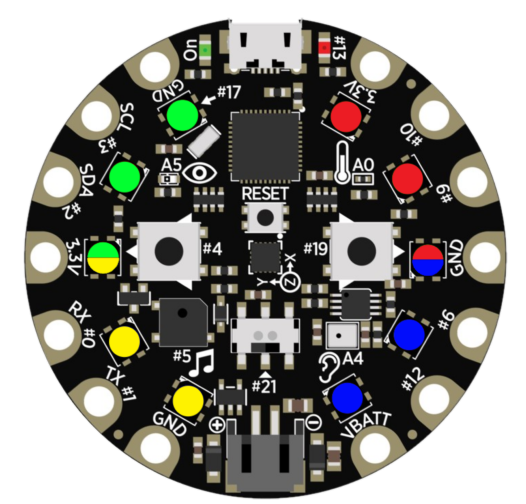
\includegraphics[width = 0.5\textwidth]{Correct_LEDs.png}
    \caption{LED Quadrants}
    \label{fig:LED_Quadrants}
\end{figure}
For example, if the user is in round four and the first four numbers in the pattern were pattern = [1,3,3,2], then the pattern displayed would be: green, blue, blue, yellow.
\vspace*{0.5cm}
\\
%Checking the User Input
Next, the user input and validation building bock was created. To accept the user input, a while loop was created to run while the number of user inputs is less than the current round number. While in this loop, the circuit playground express monitors each of the capacitive touch sensors. If the capacitive touch sensors in any of the four quadrants is above a predetermined threshold, then that quadrant's LEDs are illuminated the proper color, the corresponding quadrant sound is played, and the number associated with that quadrant is saved to a user input vector. Once an input has been collected, the variable "time\_to\_check" is set to 1, indicating that the most recent addition to the input vector needs to be checked with the pattern vector. If the pattern is correct, then "time\_to\_check" is set back to zero and the next input can be collected until the input count is equal to the round number. At this point in development, the game would simply stop if the user submitted an incorrect input or successfully matched the entire pattern. To make the game more enjoyable, further features were added. One of these features improved the experience if the user did not enter the correct pattern.
\subsubsection{Development of Additional Features}
%Incorrect User Input
Instead of simply stopping the game without any feedback to the user, an incorrect pattern building block was created. The desire for this segment of code was twofold: to indicate to the user that an incorrect pattern was submitted and show the user which quadrant was expected. To achieve this, the if statement for an incorrect input was built upon, first with all ten LEDs illuminating red for one second. A moment after the LEDs are illuminated, a linearly decreasing tone is played on the speaker. For reference, the tone is similar to the sound that is made when Bowser is knocked down in Super Mario Bros. The LEDs are cleared, followed by an if statement that illuminates the correct quadrant's LEDs and tone three times, each time for a quarter of a second. The game then returns to the game start loop. This improvement allows the user to not only immediately know they lost the game but also know which quadrant they should have selected.
\vspace*{0.5cm}
\\
%Correct User Input to Win the Game
Another desirable feature is incorporating a special sequence if the user wins the game by correctly matches the entire pattern. This sequence is indicated as described above and is shown by the variable win\_condition. When the win\_condition variable is set to 1, the win condition if statement is activated. First, all LEDs are illuminated using the setPixelColor function, with the win sounds playing moments later. The win noises are similar to a shortened version of what would play on a trumpet when a king arrives. After the victory tones are played, a for loop is triggered that sets the LEDs to rainbow colors that change every 350 milliseconds.
%Sound and difficulty settings that were added later
\vspace*{0.5cm}
\\
The final additional feature was the difficulty setting. The difficulty setting was designed to make the game harder by displaying the pattern quicker and increasing the total pattern length. To choose the difficulty, the user first moves the slide switch to the left. This activates the difficulty selection loop and illuminates the upper left LED green. While the slide switch is to the left, the user can press the left button to trigger the if statement that reduces the difficulty or visa versa with the right button. In total, there are ten difficulties ranging from 1 to 11. The current difficulty is indicated to the user by an illuminated LED. For each increase in difficulty, the lit LED also increases, starting at the upper left corner and going counterclockwise. The difficulty is saved to a variable, which is then used to calculate the pattern display time and the total pattern length. At the easiest difficulty, the game is ten rounds, where the hardest difficulty is twenty rounds.
\section{STATUS} % ASHLEY
%Here,  you need to honestly assess what the status of the project is.  If successful, state that it was successful and all the goals that it achieved (your goals are from your project proposal).  If not successful, state what was completed, what was not completed and state what happened.

The code for the Simon device was successfully developed and the device itself is operational. All goals discussed in the original proposal were achieved.

\subsection{Lessons Learned} % ASHLEY
%Here, put any lessons learned from this project.  This may also relate to some of the items that you did not accomplish with this project.

%OTHER IDEAS FROM LOGAN: 
%-Could talk about how the random function needs to be seeded first to properly create random numbers
%-How we needed to set a threshold for the capacitive touch sensors so they would only recognise true touches. Currently the threshold is about 285, unsure on the units

One constraint that was considered during development was a time limit on the player input after the desired sequence is displayed. This constraint was not included in the final product due to the difficulty of running several constraints simultaneously.

\section{RESULTS} % ASHLEY
%Put all results here.  If you collected data, explain and show at least some analysis on the data you collected.  If no data is collected, you should have collected reactions from others using your device and put that feedback here.  Any graphs you generated should be here as well.  You must include a copy of your source code in the appendix.  There is an example of this below.  Also, include the link to your GitHub repository.  You can use the \verb=\url=  command like this \url{https://github.com/AerE-361-FinalProject/Project-Report-AerE-361}.

The initial working code for the Simon game seemed perfect on the computer, but failed to please our test subjects. The game would originally show the color sequence at a very slow pace, leaving the person using the device to forget the color sequence before it was even done flashing. This problem was solved by having the color sequence speed up as the game goes on. This feature was tweaked across all difficulties to make the game more enjoyable.

\section{FUTURE WORK} % JAROD
%Your future work includes what your team would continue to improve on and change if you had more time.  This could be expanding additional features or fixing something that you couldn't figure out.  It helps to explain at least a little on what you would plan to do to improve your product.

If the team were allowed more time to develop the project, some additional features would be including a more diverse variety of inputs for the sequences, and we would also include an expiration timer after each input. The expiration timer would begin after the leading sequence was finished, and also after each user input to ensure that the user would interact within an appropriate time. Some additional input variations would be a clap into the microphone, or requiring a certain accelerometer reading to be achieved through shaking the Circuit Playground Express device.

\section{CONCLUSION} % CHARLES
In conclusion, we discussed many of the features and inspiration for our device.  We covered the solution to our problem statement through the code's development, development of additional features and explained the gameplay for the device. Finally, we reported the current status of or project as well as some future things we can work on.  We are happy to report that we successfully were able to create a device that solve or COVID-19 related boredom that matches the features of the original Simon game coupled with our own spin and ingenuity.

\newpage
\bibliographystyle{plain}
\bibliography{ref}
\newpage
% you need to have at least your code in your appendix
\appendix

\section{SOURCE CODE}
%Source Code
%\lstinputlisting[language=Arduino]{demo.ino}
\tiny
\begin{lstlisting}[language=Arduino]
#include <Adafruit_CircuitPlayground.h>

uint8_t pixeln = -1;
bool slideSwitch;
int selected_difficulty = 1; //Sets the difficulty to 1 upon startup

void setup() {
  // put your setup code here, to run once:
  Serial.begin(9600);
  randomSeed(analogRead(2));
  CircuitPlayground.begin();
}

void loop() {
  while (1==1){ //Continuous loop that checks for the beginning of a game
      slideSwitch = CircuitPlayground.slideSwitch();

  if (CircuitPlayground.slideSwitch() == 1)
    CircuitPlayground.setPixelColor((selected_difficulty-1),(0+selected_difficulty*25),(255-selected_difficulty*25),0);
    while(CircuitPlayground.slideSwitch() == 1) 
    {
      if (CircuitPlayground.rightButton() && selected_difficulty < 10)
    {
      ++selected_difficulty;
      CircuitPlayground.clearPixels();
      CircuitPlayground.setPixelColor((selected_difficulty-1),(0+selected_difficulty*25),(255-selected_difficulty*25),0);
      delay(200);
    }

    else if (CircuitPlayground.leftButton() && selected_difficulty > 1)
    {
      --selected_difficulty;
      CircuitPlayground.clearPixels();
      CircuitPlayground.setPixelColor((selected_difficulty-1),(0+selected_difficulty*25),(255-selected_difficulty*25),0);
      delay(200);
    }
  }
    
  CircuitPlayground.clearPixels();
  if (CircuitPlayground.leftButton()&&CircuitPlayground.rightButton() && slideSwitch == 0){ //Indicating the beginning of a game
    CircuitPlayground.setPixelColor(0,CircuitPlayground.colorWheel(85));
    CircuitPlayground.setPixelColor(1,CircuitPlayground.colorWheel(85));
    CircuitPlayground.setPixelColor(2,CircuitPlayground.colorWheel(85));
    CircuitPlayground.setPixelColor(3,CircuitPlayground.colorWheel(85));
    CircuitPlayground.setPixelColor(4,CircuitPlayground.colorWheel(85));
    CircuitPlayground.setPixelColor(5,CircuitPlayground.colorWheel(85));
    CircuitPlayground.setPixelColor(6,CircuitPlayground.colorWheel(85));
    CircuitPlayground.setPixelColor(7,CircuitPlayground.colorWheel(85));
    CircuitPlayground.setPixelColor(8,CircuitPlayground.colorWheel(85));
    CircuitPlayground.setPixelColor(9,CircuitPlayground.colorWheel(85));

    //Begin game sounds
    CircuitPlayground.playTone(262, 200); //C4
    CircuitPlayground.playTone(220, 100); //A3
    CircuitPlayground.playTone(262, 100); //C4
    CircuitPlayground.playTone(392, 100); //G4
    delay(500);
    CircuitPlayground.clearPixels();
    
    //Defining Variables
      int input_count = 0;      //Variable that tracks inputs within a round
      int display_count = 0;    //Counter that indicates which index in the patter to display to the user
      int round_input = 1;      //Counter that indicates the current round
      int time_to_check = 0;    //Indicator that allows a user input to be checked with the correct pattern
      int input_vect[20];       //Initializing the vector that the user input is saved to
      int end_game = 0;         //Variable that is set to 1 when it is the end of the game
      int win_condition = 0;    //Variable that is set to 1 if you win the game
    //Time Variables
      float display_time = 500;     //Default display time is 500 milliseconds
      float max_display_time = 500; //Maximum time the color of the pattern will be displayed.  Also is the length of the break afterwards
      float min_display_time = 100; //Minimum time the color of the pattern will be displayed.  Also is the length of the break afterwards
    
    //Set Difficulty
      int game_length = 9 + selected_difficulty; //defult game length is 10 rounds
      max_display_time = max_display_time - (200.0) * (((float)selected_difficulty - 1.0) / 9.0);

    // Random Number Generator for Pattern Array
    int pattern[20]; //Array of 20 random numbers between 1:4

    for (int i = 0; i < game_length; i++){
     pattern[i] = random(1,5); //Fill pattern array with random numbers 1:4 upper bound is exclusive
    }

    while(end_game == 0 && win_condition == 0) //Loop that runs while the game is progressing (ie not won or lost)
    {
      display_count = 0;
      input_count = 0;
      
      delay(1000);
      
      while((display_count < round_input) && round_input <= game_length) //Loop to display the pattern to the user
      {
        // Set Display Time Based on Game Length
        display_time = min_display_time + (max_display_time - min_display_time)*(((float)game_length - (float)round_input)/((float)game_length - 1.0)); //Decrease display_time based on the round number
        
        if(pattern[display_count] == 1) //Quadrant 1: Green
        {
          CircuitPlayground.setPixelColor(0,CircuitPlayground.colorWheel(85));
          CircuitPlayground.setPixelColor(1,CircuitPlayground.colorWheel(85));
          CircuitPlayground.setPixelColor(2,CircuitPlayground.colorWheel(85));
          CircuitPlayground.playTone(196, display_time); //G4
          CircuitPlayground.clearPixels();
          delay(display_time);
        }
        else if (pattern[display_count] == 2) //Quadrant 2: Yellow
        {
          CircuitPlayground.setPixelColor(2,255,255,0);
          CircuitPlayground.setPixelColor(3,255,255,0);
          CircuitPlayground.setPixelColor(4,255,255,0);
          CircuitPlayground.playTone(277, display_time); //C#4
          CircuitPlayground.clearPixels();
          delay(display_time);
        }
        else if (pattern[display_count] == 3) //Quadrant 3: Blue
        {
          CircuitPlayground.setPixelColor(5,CircuitPlayground.colorWheel(170));
          CircuitPlayground.setPixelColor(6,CircuitPlayground.colorWheel(170));
          CircuitPlayground.setPixelColor(7,CircuitPlayground.colorWheel(170));
          CircuitPlayground.playTone(330, display_time); //E4
          CircuitPlayground.clearPixels();
          delay(display_time);
        }
        else if (pattern[display_count] == 4) //Quadrant 4: Red
        {
          CircuitPlayground.setPixelColor(7,CircuitPlayground.colorWheel(0));
          CircuitPlayground.setPixelColor(8,CircuitPlayground.colorWheel(0));
          CircuitPlayground.setPixelColor(9,CircuitPlayground.colorWheel(0));
          CircuitPlayground.playTone(220, display_time); //A3
          CircuitPlayground.clearPixels();
          delay(display_time);
        }
        ++display_count;
      }
      
      while(input_count < round_input) //Loop to accept the user input
      {
        
      if (CircuitPlayground.readCap(3) > 285 || CircuitPlayground.readCap(2) > 285) //Quadrant 1
      {
        CircuitPlayground.setPixelColor(0,CircuitPlayground.colorWheel(85));
        CircuitPlayground.setPixelColor(1,CircuitPlayground.colorWheel(85));
        CircuitPlayground.setPixelColor(2,CircuitPlayground.colorWheel(85));
        CircuitPlayground.playTone(196, display_time); //G4
        CircuitPlayground.clearPixels();
        input_vect[input_count] = 1;
        time_to_check = 1;
      }
      
      else if (CircuitPlayground.readCap(0) > 300 || CircuitPlayground.readCap(1) > 300) //Quadrant 2
      {
        CircuitPlayground.setPixelColor(2,255,255,0);
        CircuitPlayground.setPixelColor(3,255,255,0);
        CircuitPlayground.setPixelColor(4,255,255,0);
        CircuitPlayground.playTone(277, display_time); //C#4
        CircuitPlayground.clearPixels();
        input_vect[input_count] = 2;
        time_to_check = 1;
      }
      
      else if (CircuitPlayground.readCap(12) > 285 || CircuitPlayground.readCap(6) > 285) //Quadrant 3
      {
        CircuitPlayground.setPixelColor(5,CircuitPlayground.colorWheel(170));
        CircuitPlayground.setPixelColor(6,CircuitPlayground.colorWheel(170));
        CircuitPlayground.setPixelColor(7,CircuitPlayground.colorWheel(170));
        CircuitPlayground.playTone(330, display_time); //E4
        CircuitPlayground.clearPixels();
        input_vect[input_count] = 3;
        time_to_check = 1;
      }
      
      else if (CircuitPlayground.readCap(9) > 285 || CircuitPlayground.readCap(10) > 285) //Quadrant 4
      {
        CircuitPlayground.setPixelColor(7,CircuitPlayground.colorWheel(0));
        CircuitPlayground.setPixelColor(8,CircuitPlayground.colorWheel(0));
        CircuitPlayground.setPixelColor(9,CircuitPlayground.colorWheel(0));
        CircuitPlayground.playTone(220, display_time); //A3
        CircuitPlayground.clearPixels();
        input_vect[input_count] = 4;
        time_to_check = 1;
      }
      
      if (time_to_check == 1 && input_vect[input_count] != pattern[input_count]) //If user input is not correct
        {
          //Display Red on all LEDs for 1 second
          CircuitPlayground.setPixelColor(0,CircuitPlayground.colorWheel(0));
          CircuitPlayground.setPixelColor(1,CircuitPlayground.colorWheel(0));
          CircuitPlayground.setPixelColor(2,CircuitPlayground.colorWheel(0));
          CircuitPlayground.setPixelColor(3,CircuitPlayground.colorWheel(0));
          CircuitPlayground.setPixelColor(4,CircuitPlayground.colorWheel(0));
          CircuitPlayground.setPixelColor(5,CircuitPlayground.colorWheel(0));
          CircuitPlayground.setPixelColor(6,CircuitPlayground.colorWheel(0));
          CircuitPlayground.setPixelColor(7,CircuitPlayground.colorWheel(0));
          CircuitPlayground.setPixelColor(8,CircuitPlayground.colorWheel(0));
          CircuitPlayground.setPixelColor(9,CircuitPlayground.colorWheel(0));
          for (int i = 0; i < 10; ++i)
          {
            CircuitPlayground.playTone((700-50*i), 20);
          }
          delay(800);
          CircuitPlayground.clearPixels();
          
          //Now flash the expected quadrant's LEDs 3 times
          if (pattern[input_count] == 1) //If quadrant 1 was expected
          {
            for (int j = 0; j < 3; ++j)
            {
              CircuitPlayground.setPixelColor(0,CircuitPlayground.colorWheel(85));
              CircuitPlayground.setPixelColor(1,CircuitPlayground.colorWheel(85));
              CircuitPlayground.setPixelColor(2,CircuitPlayground.colorWheel(85));
              CircuitPlayground.playTone(196, 250); //G4
              CircuitPlayground.clearPixels();
              delay(250);
            }
          }
          
          else if (pattern[input_count] == 2) //If quadrant 2 was expected
          {
            for (int j = 0; j < 3; ++j)
            {
              CircuitPlayground.setPixelColor(2,255,255,0);
              CircuitPlayground.setPixelColor(3,255,255,0);
              CircuitPlayground.setPixelColor(4,255,255,0);
              CircuitPlayground.playTone(277, 250); //C#4
              CircuitPlayground.clearPixels();
              delay(250);
            }
          }
          
          else if (pattern[input_count] == 3) //If quadrant 3 was expected
          {
            for (int j = 0; j < 3; ++j)
            {
              CircuitPlayground.setPixelColor(5,CircuitPlayground.colorWheel(170));
              CircuitPlayground.setPixelColor(6,CircuitPlayground.colorWheel(170));
              CircuitPlayground.setPixelColor(7,CircuitPlayground.colorWheel(170));
              CircuitPlayground.playTone(330, 250); //E4
              CircuitPlayground.clearPixels();
              delay(250);
            }
          }
          
          else if (pattern[input_count] == 4) //If quadrant 4 was expected
          {
            for (int j = 0; j < 3; ++j)
            {
              CircuitPlayground.setPixelColor(7,CircuitPlayground.colorWheel(0));
              CircuitPlayground.setPixelColor(8,CircuitPlayground.colorWheel(0));
              CircuitPlayground.setPixelColor(9,CircuitPlayground.colorWheel(0));
              CircuitPlayground.playTone(220, 250); //A3
              CircuitPlayground.clearPixels();
              delay(250);
            }
          }
          
          end_game = 1; //Allows us to exit the game execution loop
          break;
        }
        
        else if (time_to_check == 1 && input_vect[input_count] == pattern[input_count]) //If input is correct
        {
        ++input_count;
        time_to_check = 0;
        }
        
      }
      //All inputs are correct and it is not the end of the game: increase round
      if(end_game == 0)
      {
        round_input = round_input + 1;
      }
      
      if (round_input-1 == game_length) //User successfully passed all rounds, indicate win by setting win_condition to 1
      {
        win_condition = 1;
      }
      
    }
    
    if (win_condition == 1) //If user won the game
      {
        //Flash all LEDs Green
        CircuitPlayground.setPixelColor(0,CircuitPlayground.colorWheel(85));
        CircuitPlayground.setPixelColor(1,CircuitPlayground.colorWheel(85));
        CircuitPlayground.setPixelColor(2,CircuitPlayground.colorWheel(85));
        CircuitPlayground.setPixelColor(3,CircuitPlayground.colorWheel(85));
        CircuitPlayground.setPixelColor(4,CircuitPlayground.colorWheel(85));
        CircuitPlayground.setPixelColor(5,CircuitPlayground.colorWheel(85));
        CircuitPlayground.setPixelColor(6,CircuitPlayground.colorWheel(85));
        CircuitPlayground.setPixelColor(7,CircuitPlayground.colorWheel(85));
        CircuitPlayground.setPixelColor(8,CircuitPlayground.colorWheel(85));
        CircuitPlayground.setPixelColor(9,CircuitPlayground.colorWheel(85));

        //Play win sounds
        CircuitPlayground.playTone(440, 100); //A4
        CircuitPlayground.playTone(523, 100); //C5
        CircuitPlayground.playTone(784, 100); //G5
        CircuitPlayground.playTone(1047, 250); //C6

        for(int i = 1; i <= 15; ++i)
          {
            CircuitPlayground.setPixelColor(0,CircuitPlayground.colorWheel(25*i));
            CircuitPlayground.setPixelColor(1,CircuitPlayground.colorWheel(25*i));
            CircuitPlayground.setPixelColor(2,CircuitPlayground.colorWheel(25*i));
            CircuitPlayground.setPixelColor(3,CircuitPlayground.colorWheel(25*i*2));
            CircuitPlayground.setPixelColor(4,CircuitPlayground.colorWheel(25*i*2));
            CircuitPlayground.setPixelColor(5,CircuitPlayground.colorWheel(25*i*3));
            CircuitPlayground.setPixelColor(6,CircuitPlayground.colorWheel(25*i*3));
            CircuitPlayground.setPixelColor(7,CircuitPlayground.colorWheel(25*i*3));
            CircuitPlayground.setPixelColor(8,CircuitPlayground.colorWheel(25*i*4));
            CircuitPlayground.setPixelColor(9,CircuitPlayground.colorWheel(25*i*4));
            delay(350);
            CircuitPlayground.clearPixels();
          }
        win_condition = 0;
      }
  }
  }
}
\end{lstlisting}

\end{document}